\documentclass[border=3pt]{standalone}
\usepackage{tikz}
\usepackage{amsmath,amssymb}

\definecolor{qqqqff}{RGB}{1,82,142}
\definecolor{maincolor2}{RGB}{21,182,184}

\begin{document}
	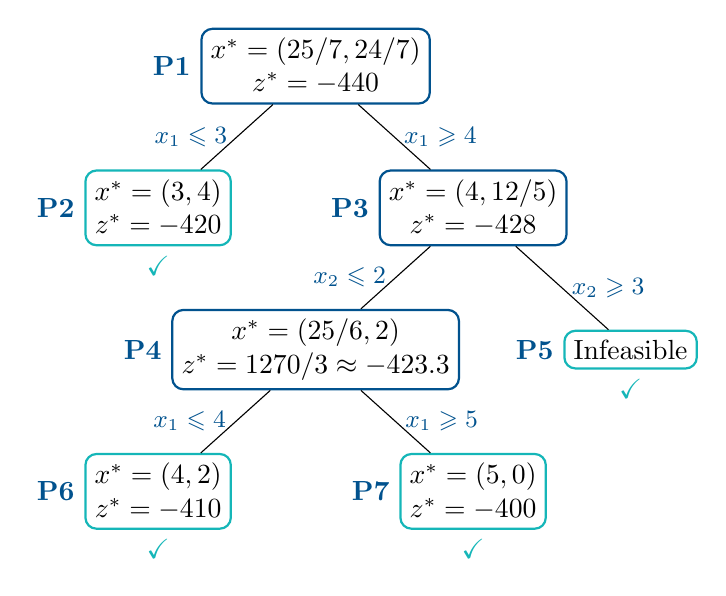
\begin{tikzpicture}[
		sibling distance=4cm,
		level distance=1.8cm,
		treenode/.style={shape=rectangle, rounded corners, align=center, draw=qqqqff, thick},
		solnode/.style={shape=rectangle, rounded corners, align=center, draw=maincolor2, thick},
		edge label/.style={font=\small, color=qqqqff},
		every edge/.style={draw=qqqqff, thick}
		]
		\node[treenode, label=west:\textcolor{qqqqff}{\textbf{P1}}] {$x^* = (25/7,24/7)$ \\ $z^* = -440$}
		child {node[solnode, label=west:\textcolor{qqqqff}{\textbf{P2}}, label=south:\textcolor{maincolor2}{$\checkmark$}] {$x^* = (3,4)$ \\ $z^* = -420$}
			edge from parent node [left, edge label] {$x_1 \leqslant 3$}
		}
		child {node[treenode, label=west:\textcolor{qqqqff}{\textbf{P3}}] {$x^* = (4,12/5)$ \\ $z^* = -428$}
			child {node[treenode, label=west:\textcolor{qqqqff}{\textbf{P4}}] {$x^* = (25/6,2)$ \\ $z^* = 1270/3 \approx -423.3$}
				child {node[solnode, label=west:\textcolor{qqqqff}{\textbf{P6}}, label=south:\textcolor{maincolor2}{$\checkmark$}] {$x^* = (4,2)$ \\ $z^* = -410$}
					edge from parent node [left, edge label] {$x_1 \leqslant 4$}
				}
				child {node[solnode, label=west:\textcolor{qqqqff}{\textbf{P7}}, label=south:\textcolor{maincolor2}{$\checkmark$}] {$x^* = (5,0)$ \\ $z^* = -400$}
					edge from parent node [right, edge label] {$x_1 \geqslant 5$}
				}
				edge from parent node [left, edge label] {$x_2 \leqslant 2$}
			}
			child {node[solnode, label=west:\textcolor{qqqqff}{\textbf{P5}}, label=south:\textcolor{maincolor2}{$\checkmark$}] {Infeasible}
				edge from parent node [right, edge label] {$x_2 \geqslant 3$}
			}
			edge from parent node [right, edge label] {$x_1 \geqslant 4$}
		};
	\end{tikzpicture}
\end{document}